\section{Combining models and net-of-cost production results}
\label{sec:models}

\subsection{The Fama--MacBeth production combiner}
\label{sec:fm}

The production question --- one ranking merging the surviving 13F
signals with classical characteristics --- was raced across three
combining schools on identical quarters, strictly out-of-sample
(expanding estimates, twelve-quarter warm-up). Predictors,
pre-registered: size, momentum, beta, low-volatility, short-term
reversal, liquidity, plus NCB, breadth change, FSS, and flow
pressure, all as centered cross-sectional percentile ranks.

\begin{itemize}
\item \textbf{A. Fama--MacBeth/Lewellen} (per-quarter cross-sectional
  OLS premia, expanding mean, $E[r]=\bar\lambda'x$): spread
  $+5.4\%$/q ($t=+2.65$), \textbf{Sharpe 0.86}, IC $+0.030$.
\item \textbf{B. IC-weighted composite} (Grinold--Kahn): $+4.3\%$/q,
  Sharpe 0.69 --- univariate weights ignore signal overlap.
\item \textbf{C. Naive rank average} (NCB $+$ FSS only): $+2.6\%$/q,
  Sharpe 0.74. Paired deltas: A$-$B $t=+1.18$; A$-$C $t=+1.96$.
\end{itemize}

The joint-marginality table is the deliverable the one-at-a-time
factor ladder cannot produce: holding all ten predictors
simultaneously, NCB's premium is $t=+3.04$ and breadth change's
$t=+4.01$ --- the 13F premia are marginal to six classical
characteristics at once. Breadth change is the canonical example of
an \emph{ingredient}: weak as a standalone quintile sort
(Table~\ref{tab:catalogue}) yet the second-strongest joint premium;
signals correlated with controls reveal their value only in the
joint estimate. Figure~\ref{fig:race} shows the race cumulatively.

\begin{figure}[t]
\centering
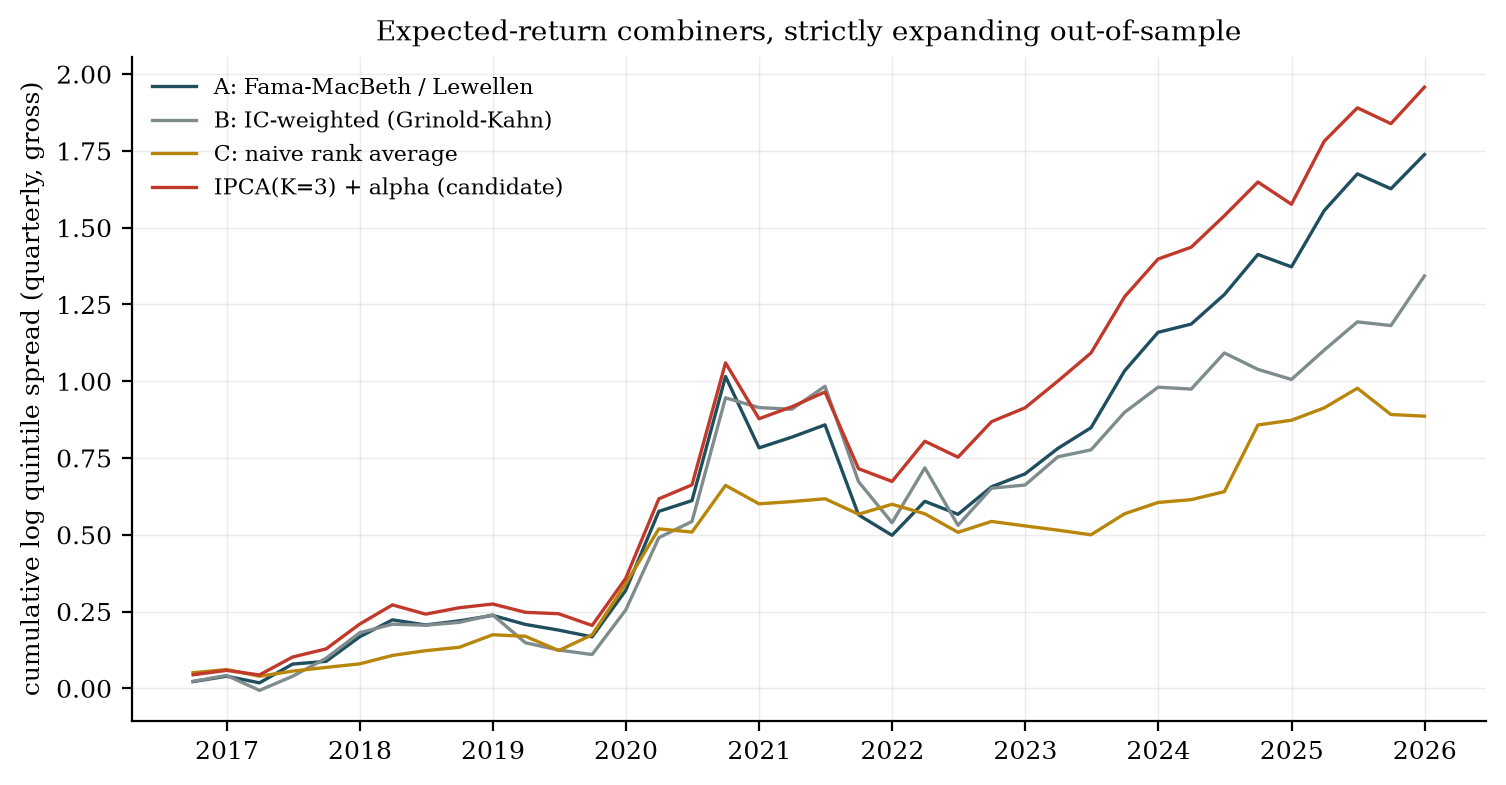
\includegraphics[width=.85\linewidth]{figs/f2_combiner_race.png}
\caption{Expected-return combiners, strictly expanding OOS, gross
quintile spreads (log cumulative). The Fama--MacBeth combiner is the
production model; the IPCA challenger is a candidate under the
funnel's promotion rules.}
\label{fig:race}
\end{figure}

\subsection{The IPCA challenger: is the premium a latent-factor loading?}
\label{sec:ipca}

Under \citet{kps2019}, factor loadings are instrumented by
characteristics ($\beta_{i,t}=z_{i,t}'\Gamma$) and estimated jointly
with latent factors by alternating least squares; our implementation
was verified line-by-line against the authors' reference package
($N_t$-weighted $\Gamma$ step, intercept as pre-specified factor,
$W_\alpha$ wild bootstrap with $t(5)$ multipliers, 500 draws). Fifty
quarters, instruments $=$ constant $+$ the ten predictors. Results:
total $R^2$ 0.10--0.12 at $K=1..4$; the formal $W_\alpha$ test does
not reject $\Gamma_\alpha=0$ ($p=0.41$--$0.59$ --- expected at
$T=50$; the test needs hundreds of periods for power); the
interpretable spanning statistic --- the time-series alpha of the
NCB-managed portfolio on the latent factors --- is $t\approx+6$ at
every $K$. Out-of-sample, the unrestricted forecast
$z'(\Gamma_\beta\bar\lambda + \Gamma_\alpha)$ posts Sharpe 0.97 and
beats the FM combiner paired ($+0.55\%$/q, $t=+2.08$); the genuinely
rank-restricted forecast ($z'\Gamma\bar\lambda$) ties FM
($t=-0.75$).

Two disciplines govern the reading. Algebraically, the unrestricted
unconditional forecast is \emph{not} rank-compressed
($\Gamma_\alpha$ is a free vector, so
$\Gamma_\beta\bar\lambda+\Gamma_\alpha$ spans $\mathbb{R}^{11}$): the
gain over FM comes from a different, pooled, structure-regularized
estimator of the same premia --- not from ``compression keeping the
alpha,'' and the leg that is genuinely compressed confirms this by
not beating FM. Procedurally, IPCA entered after the race was
scored: a post-hoc fourth entrant at $t=+2.08$ does not clear the
pre-registered promotion bar ($2.57$), so \textbf{FM remains the
production combiner} and IPCA+alpha is recorded as the best point
estimate on the protocol, pending fresh sample. What survives
unconditionally is the answer to ``is NCB beta in disguise?'': no
latent factor instrumentable by these characteristics absorbs it.

\subsection{The net engine}
\label{sec:engine}

Research spreads are gross and frictionless by construction; the
engine is neither. Every panel --- survivors and rejected signals
entered \emph{inverted}, so a positive net Sharpe means ``the
research conclusion pays'' --- runs through one realistic long-short
book: tradability filters (\$4 price, \$5M median dollar volume, 252
days of history), 20\% tails with a 40-name minimum per leg,
rebalanced at each signal's own decision dates, \textbf{5 bps per
side commissions} and \textbf{50 bps p.a.\ borrow on short legs},
daily net returns.

The cost assumptions are justified by the trading profile rather
than asserted. Five basis points per side is in line with realized
all-in commission-plus-spread costs for institutional trading of
liquid US equities, and this strategy is the easy case: quarterly
rebalancing (measured one-way turnover of $3$--$7\times$ per year,
Table~\ref{tab:engine}), no intraday urgency, and an explicit
liquidity control --- the tradability filter plus the per-leg
breadth minimum keeps individual positions small relative to ADV,
which is what keeps slippage beyond the flat fee second-order.
Market impact matters at scale and belongs to the capacity
discussion, not the backtest. Borrow at 50 bps p.a.\ is
general-collateral; because the FSS leg skews illiquid we report the
hard-to-borrow sensitivity: at 200 bps the FSS leg loses
$\approx1.5\%$/yr (Sharpe $0.85\to0.73$) and the combo
$\approx0.75\%$/yr (Sharpe $\approx0.9$) --- the conclusions
survive. The NCB$+$FSS book weights the two legs' ranks
\emph{equally by design}: the no-optimization default, chosen so the
production book inherits no tuned parameter; any data-driven leg
weighting would require its own surface under the
Section~\ref{sec:ncb-surface} protocol.

Table~\ref{tab:engine} reports the full battery
--- annualized net return, volatility, Sharpe, information ratio
against the hedged benchmark, maximum drawdown, Calmar, hit ratio ---
for the headline strategies on the expanded universe, and
Figure~\ref{fig:engine} the cumulative net curves. The engine
compresses everything (costs, the stricter universe, no shorting of
the illiquid tail), the ordering matches the research layer, and the
research-rejected signals inverted earn approximately zero net ---
the engine confirming, from the cost side, that the funnel's
rejections were correct.

\begin{table}[t]
\centering\footnotesize
\caption{Production-engine results, net of 5 bps/side commissions and 50 bps p.a.\ borrow on short legs; expanded universe; tradability filters \$4 / \$5M ADV / 252d. ``cost'' is the measured annualized commission drag (net run minus zero-fee run); ``turn'' the implied one-way annual turnover (traded notional over book, per year). Research-rejected signals enter inverted, so a positive Sharpe means the research conclusion prices.}
\label{tab:engine}
\begin{tabular}{lrrrrrrrr}
\toprule
strategy & ann.\ net & vol & Sharpe & maxDD & Calmar & hit & cost (bps/y) & turn \\
\midrule
NCB (residualized) & +2.9\% & 6.7\% & +0.42 & -18.7\% & +0.15 & 51\% & 65 & 6.5x \\
FM score (10 predictors) & +4.0\% & 16.9\% & +0.24 & -62.1\% & +0.06 & 51\% & 43 & 4.3x \\
NCB+FSS book & +6.2\% & 6.0\% & +1.02 & -10.6\% & +0.58 & 53\% & 67 & 6.7x \\
FSS short leg & +10.4\% & 12.2\% & +0.85 & -26.1\% & +0.40 & 54\% & 65 & 6.5x \\
dBreadth (common filers) & +1.4\% & 11.1\% & +0.13 & -28.2\% & +0.05 & 53\% & 61 & 6.1x \\
NCB v2 (catalogue spec) & +2.6\% & 8.3\% & +0.31 & -26.2\% & +0.10 & 53\% & 50 & 5.0x \\
Conviction top (level) & +2.5\% & 12.3\% & +0.20 & -49.6\% & +0.05 & 52\% & 33 & 3.3x \\
ICA reversal & -2.1\% & 8.2\% & -0.26 & -24.7\% & -0.09 & 49\% & 51 & 5.1x \\
SSI (inverted) & -2.0\% & 9.9\% & -0.20 & -34.8\% & -0.06 & 48\% & 29 & 2.9x \\
NMF crowding (inverted) & +0.7\% & 11.9\% & +0.06 & -51.4\% & +0.01 & 53\% & 45 & 4.5x \\
\bottomrule
\end{tabular}
\end{table}

\begin{figure}[t]
\centering
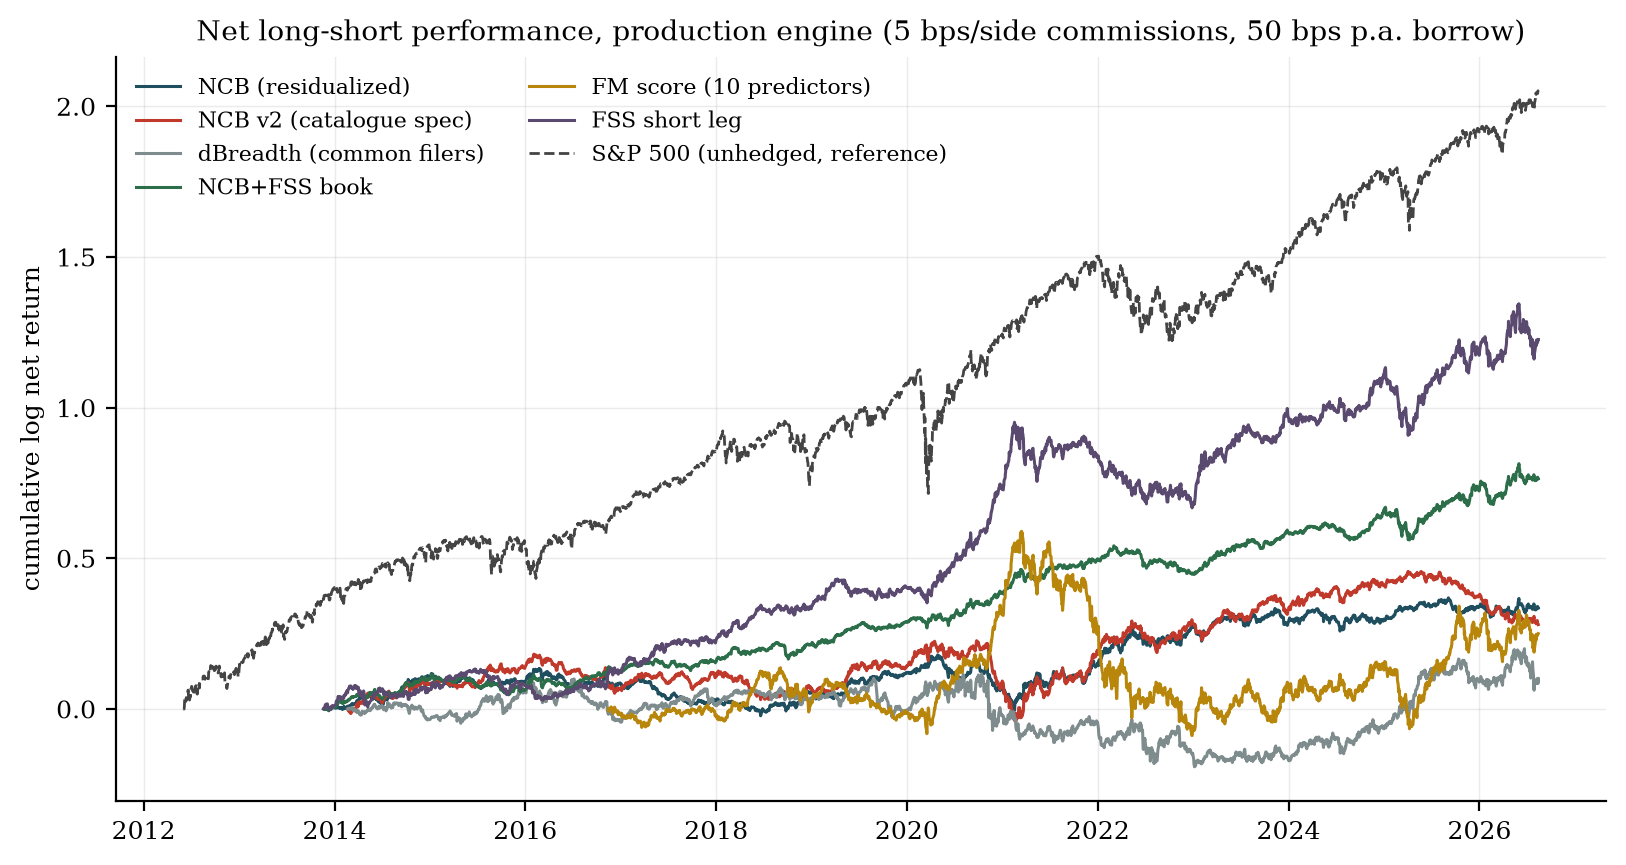
\includegraphics[width=.95\linewidth]{figs/f1_engine_curves.png}
\caption{Net long-short performance in the production engine
(log cumulative returns; 5 bps/side commissions, 50 bps p.a.\
borrow).}
\label{fig:engine}
\end{figure}

\subsection{Long-only implementation}
\label{sec:lo}

A naive long-only expression --- holding the long basket
equal-weighted against the S\&P --- is condemned by the composition
arithmetic of Section~\ref{sec:funds} before any signal question
arises: the equal-weight tilt pays the Bessembinder tax that sank
the median 13F book itself. The institutional design tilts the
\emph{benchmark}: true cap weights over the top 500 names by
repaired market capitalization (10\% cap), multiplied by
$\exp\{2k(\mathrm{rank}_i - 0.5)\}$ on the NCB$+$FSS combo rank and
renormalized, quarterly, net of 5 bps/side on turnover. The
multiplicative-exponential form is the standard tilt of
index-provider factor-tilt methodologies (MSCI-style tilt indexes
multiply parent-index weights by a positive score function): it
preserves positivity and long-only feasibility by construction,
leaves unscored names at benchmark weight (rank $0.5$), and makes
the tilt strength a single interpretable dial.
The benchmark is a genuine cap-weighted model: the top 500 names by
repaired market capitalization (official S\&P constituent weights are
licensed data; historical constituent \emph{lists} are free, weights
are not), and the repair matters --- the shares-inferred cap panel
is reliable as a ranked regression control but has a corrupt tail as
portfolio weights, fixed by replacing $|z|>2.5$ outliers of a
cross-sectional $\log(\mathrm{mcap})\sim\log(\mathrm{ADV})$
regression with their fitted values. The resulting proxy tracks the
actual S\&P~500 at a 2.7\% tracking error with $-0.6\%$/yr drift ---
close enough to serve as the cap-weighted base. Table~\ref{tab:lo}
and Figure~\ref{fig:lo}: the tilt adds $+1.0$/$+2.2$/$+3.6\%$ per
year over the benchmark at tracking errors of
$1.8$/$4.0$/$6.2\%$ for $k=1/2/3$ --- an information ratio of
$0.53$--$0.58$, \emph{roughly flat in the tilt strength}, the
signature of a scalable signal rather than a lucky corner. All three
variants also clear the S\&P itself.

\begin{table}[t]
\centering\small
\caption{Long-only cap-weighted model and its combo tilts, net of
5 bps/side commissions, quarterly rebalance, 2013--2026. ``Total
ret.'' is the portfolio's full net return (long-only, $\beta\approx
1$: it contains the market); the \emph{alpha} columns are
``excess''/IR --- against the tilt's own benchmark in the top block,
against the actual S\&P~500 in the bottom block. Rel.\ maxDD: worst
peak-to-trough of the log wealth ratio versus the same reference.
No bootstrap-selected $k$ appears \emph{by design}: the tilt-strength
surface (Figure~\ref{fig:losurface}) gives no evidence that
selecting or re-selecting $k$ from history helps, and weak evidence
that it hurts --- $k$ is shipped as the conservative default
($k=1$) and scaled by the investor's tracking-error budget.}
\label{tab:lo}
\begin{tabular}{lrrrrrrrr}
\toprule
portfolio & total ret.\ (net) & vol & Sharpe & maxDD & excess & TE &
IR & rel.\ maxDD \\
\midrule
S\&P 500 (actual index) & $+14.8\%$ & $17.1\%$ & $0.86$ & $-41.1\%$
& --- & --- & --- & --- \\
cap-weighted 500 (S\&P proxy) & $+14.1\%$ & $18.0\%$ & $0.78$ &
$-44.6\%$ & --- & --- & --- & --- \\
combo tilt $k=0.5$ & $+14.6\%$ & $18.2\%$ & $0.80$ &
$-44.6\%$ & $+0.4\%$ & $0.9\%$ & $0.49$ & $-2.5\%$ \\
combo tilt $k=1$ \textbf{(shipped default)} & $+15.1\%$ & $18.4\%$
& $0.82$ & $-44.5\%$ & $+1.0\%$ & $1.8\%$ & $0.53$ & $-5.7\%$ \\
combo tilt $k=2$ & $+16.4\%$ & $19.2\%$ & $0.85$ & $-44.1\%$ &
$+2.2\%$ & $4.0\%$ & $0.57$ & $-13.7\%$ \\
combo tilt $k=3$ & $+17.7\%$ & $20.4\%$ & $0.87$ & $-43.9\%$ &
$+3.6\%$ & $6.2\%$ & $0.58$ & $-21.2\%$ \\
\midrule
benchmark vs S\&P & & & & & $-0.6\%$ & $2.7\%$ & --- & $-17.0\%$ \\
$k=1$ vs S\&P & & & & & $+0.3\%$ & $3.6\%$ & $0.09$ & $-13.6\%$ \\
$k=3$ vs S\&P & & & & & $+2.9\%$ & $7.3\%$ & $0.40$ & $-25.5\%$ \\
\bottomrule
\end{tabular}
\end{table}

\begin{figure}[t]
\centering
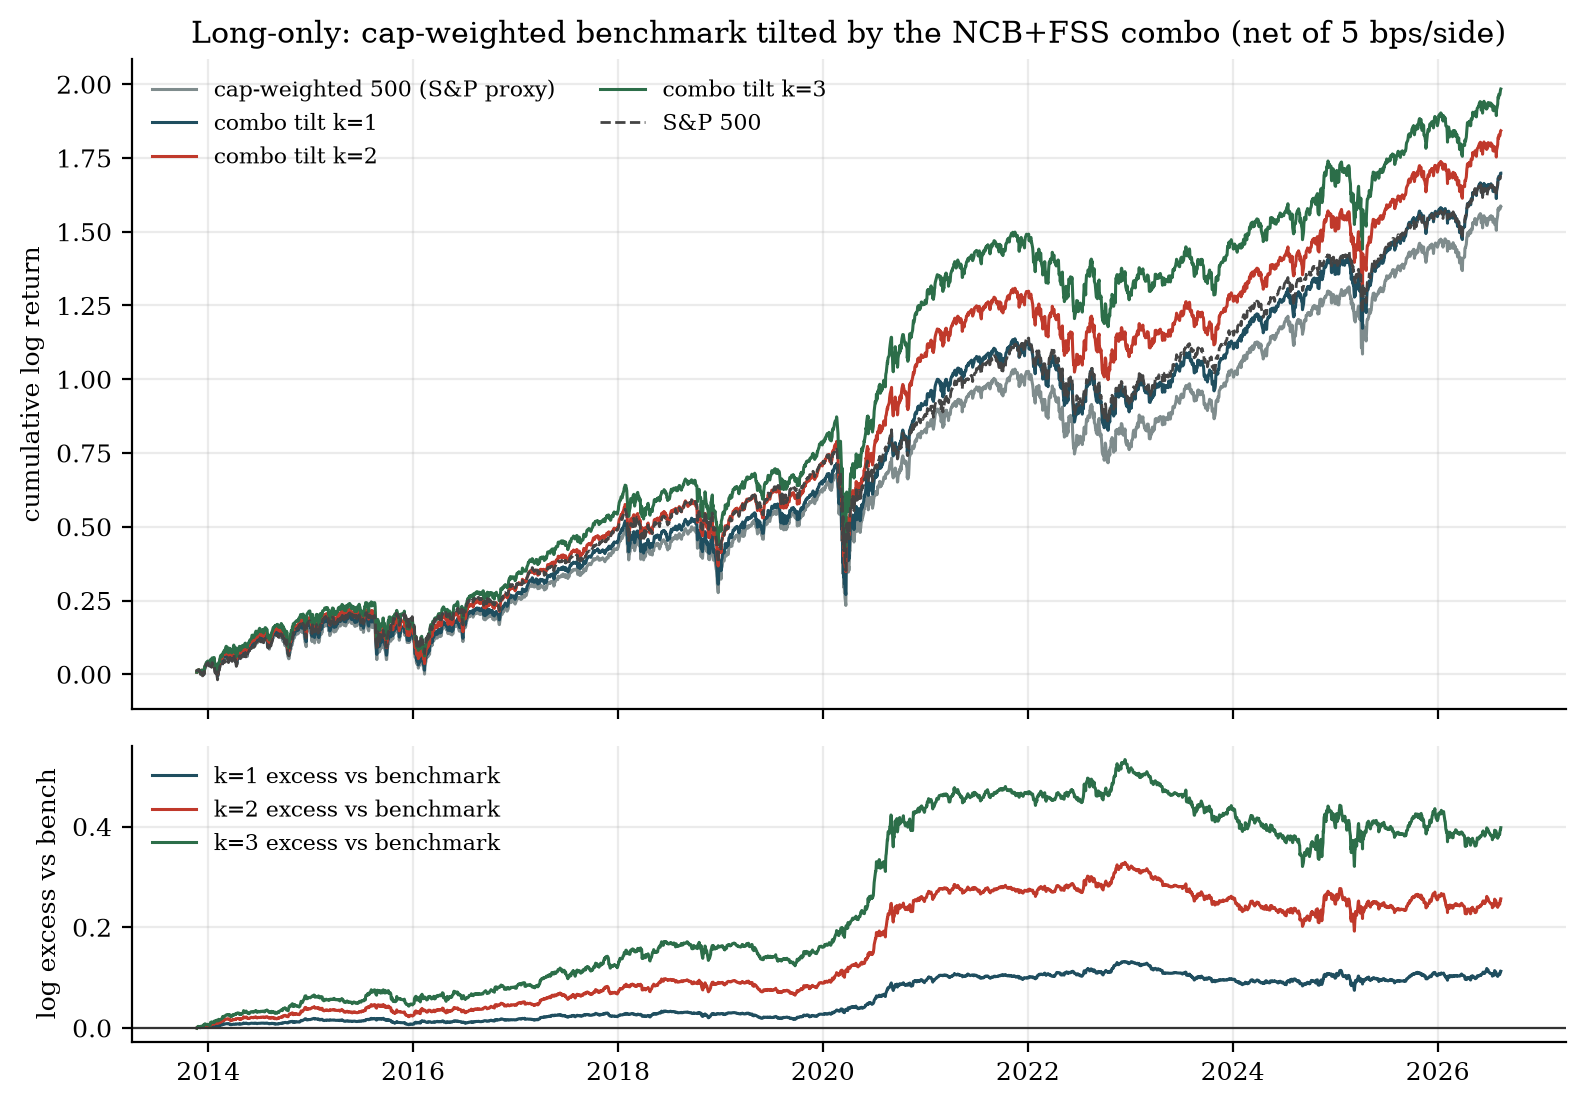
\includegraphics[width=.9\linewidth]{figs/f11_long_only.png}
\caption{Long-only benchmark tilt (log cumulative, net). Top:
levels; bottom: log excess versus the benchmark by tilt strength.}
\label{fig:lo}
\end{figure}

\paragraph{Justifying the tilt strength: the third surface.}
The one free parameter of the LO product, $k$, received the same
bootstrap treatment as the NCB and FSS specifications (grid
$k\in\{0.5,\dots,4\}$; utility $=$ IR of quarterly excess vs the
benchmark; coupled block bootstrap of the in-sample years, one IR
distribution per $k$; frozen OOS 2021--2025).
Figure~\ref{fig:losurface}: in-sample the distributions shift up
with $k$ (median IR $0.59\to1.09$; even the 5th percentile turns
positive from $k=1$) --- and in the held-out years the ordering
reverses (IR $0.42$ at $k=0.5$ down to $-0.04$ at $k=4$). Two
honesty caveats size this correctly. First, with 23 held-out
quarters the standard error of an annualized IR is $\approx 0.4$,
so the reversal is \emph{suggestive, not proven}. Second, the
mechanism is mundane: the exponential tilt is nonlinear --- large
$k$ concentrates the book far from cap weights, degrading the
transfer coefficient per unit of tracking error, and the 2021+
mega-cap regime taxed exactly that deviation. The natural objection
--- ``why not re-select $k$ each period with an expanding window?''
--- was simulated directly: an adaptive selector maximizing
expanding-window IR picks $k=4$ in essentially every quarter from
2015 through 2022 (in-sample always rewards aggression), which makes
it approximately equivalent to holding the most aggressive tilt
throughout; it earns $-0.11$ after 2021 against $+0.31$ for the
frozen default. The defensible statement is deliberately modest:
\textbf{there is no evidence that re-selecting $k$ helps, weak
evidence that it hurts, and since large $k$ buys tracking error
without reliable additional excess, the shipped default is the
conservative $k=1$} --- with $k$ treated as the investor's
tracking-error budget ($0.9\%$ at $k=0.5$, $1.8\%$ at $k=1$, $6\%$
at $k=3$), not as a fitted parameter.
Across the three applications of the \citet{oliveira2025} protocol,
one surface supported selection (NCB: IS ranks OOS at $+0.53$) and
two refused it (FSS $-0.81$, LO tilt $-1.0$) --- the protocol's
value in this project was less in picking parameters than in
\emph{detecting when picking is illegitimate}.

\begin{figure}[t]
\centering
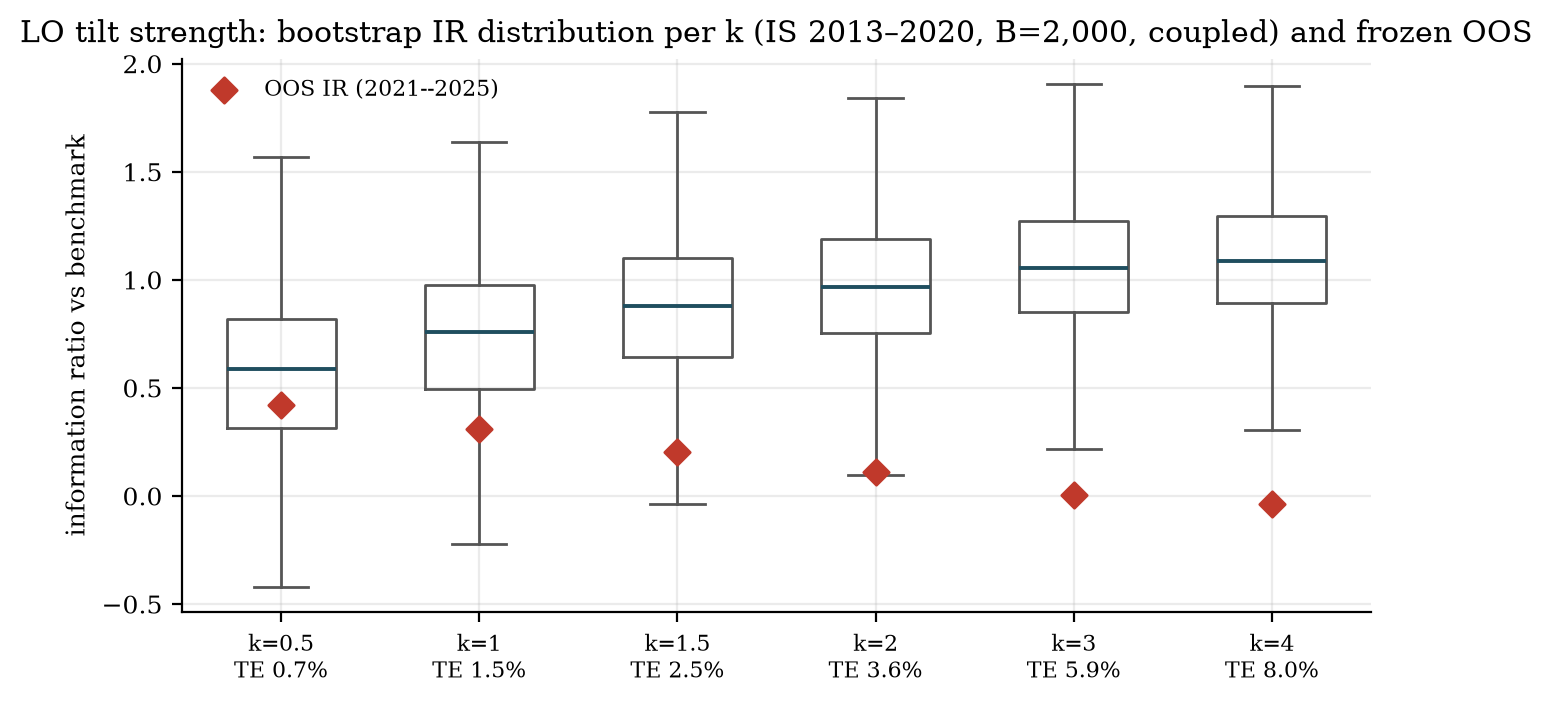
\includegraphics[width=.8\linewidth]{figs/f12_lo_surface.png}
\caption{One bootstrap IR distribution per tilt strength (boxes:
in-sample 2013--2020, coupled resamples) against the frozen held-out
IR (diamonds). The in-sample ordering reverses in the held-out years
--- suggestive at this sample size (IR s.e.\ $\approx 0.4$), and
enough to treat the tilt strength as a risk budget rather than a
fitted parameter.}
\label{fig:losurface}
\end{figure}

\paragraph{The research-to-production decomposition of the FM
combiner.} The FM combiner's research Sharpe (0.86, gross quintile
spreads on the wide $\ge$5-holder universe) does not survive the
engine (net Sharpe 0.24, $-61\%$ drawdown), and the decomposition is
a result in itself, produced by three controlled cuts. Costs are
irrelevant (0.24 with commissions, 0.26 without). The engine is
faithful (a plain quintile spread of the same ranking on the engine's
tradable universe reproduces the engine's Sharpe). What kills it is
composition: on the tradable universe the raw ranking retains
$+2.2\%$/q (Sharpe 0.41, $t=+1.32$), and residualizing the ranking
on size and liquidity leaves \emph{nothing} ($-1.1\%$/q, $t=-0.70$).
The combiner's headline premium rides its two largest lambdas ---
size ($t=+4.45$) and liquidity ($t=+4.39$) --- which pay either
outside the tradable set or as risk compensation the engine cannot
monetize. The tradable alpha inside the ranking is precisely its 13F
components, which is why the production book is NCB$+$FSS
(Table~\ref{tab:engine}: net Sharpe \textbf{1.03}, maximum drawdown
$-11\%$) rather than the full ten-characteristic ranking. The joint
FM machinery keeps its role as the \emph{measurement} device
(Section~\ref{sec:fm}); the tradable book is built from the
components that survive on the tradable universe.
